\documentclass[thesis.tex]{subfiles}
\begin{document}

\chapter{Pedestrian detection}
\label{sec:od}
In this chapter we describe the object detection problem and how we apply the discriptor to solve it.
Some introduction to object detection

Sliding window: $\sigma \cdot 134x70$ (128x64 + 3 pixel border)

\section{Support vector machine}

$L_2$-regularized $L_2$ loss support vector classifier from LIBLINEAR v. 1.94 \cite{fan2008liblinear}


\section{Performance measures}

\section{Dataset}
\label{sec:odDataset}

The dataset we use for training and testing our descriptor on the pedestrian detection application is called the \emph{INRIA Person Dataset}\footnote{\url{http://pascal.inrialpes.fr/data/human/}} (from now on called the INRIA dataset) constructed by \citet{dalal2005histograms}.
It concists of various real world images grouped into two subsets: Images with pedestrians (positives) and images without pedestrians (negatives). The positive images are rescaled cutouts centered around each pedestrian in larger images. The cutouts are first extracted and then individually re-scaled to make the pedestrian of each cutout 96 pixels in height from their feet to shoulders. The size of the cutouts are $64 \times 128$ pixels. In case a pedestrian cutout is smaller than the defined size after resizing, the borders are replicated to achieve the desired dimensions.
The positive set only contains images of somewhat upright persons that initially were at least 100 pixels in height. In order to improve the robustness of the dataset against reflected images, each positive cutout has its left-right reflected image included as well.
The training dataset has a total of 2416 positives and 1218 negative images.
The test dataset has a total of 1126 positives and 453 negative images.


\Cref{fig:inriaExampleImages} shows examples of positive \subref{fig:inriaPositives} and negative \subref{fig:inriaNegatives} images from the INRIA dataset. From the positive examples we clearly see the high variety of upright positions and surroundings in the dataset.

\begin{figure}
	\centering
	\begin{subfigure}[t]{\textwidth}
		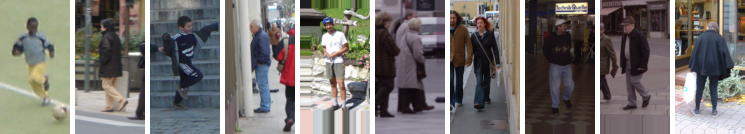
\includegraphics[width=\textwidth]{img/inriaPositives.png}
		\caption{Positives}
		\label{fig:inriaPositives}
		\vspace{2mm}
	\end{subfigure}
	\begin{subfigure}[t]{\textwidth}
		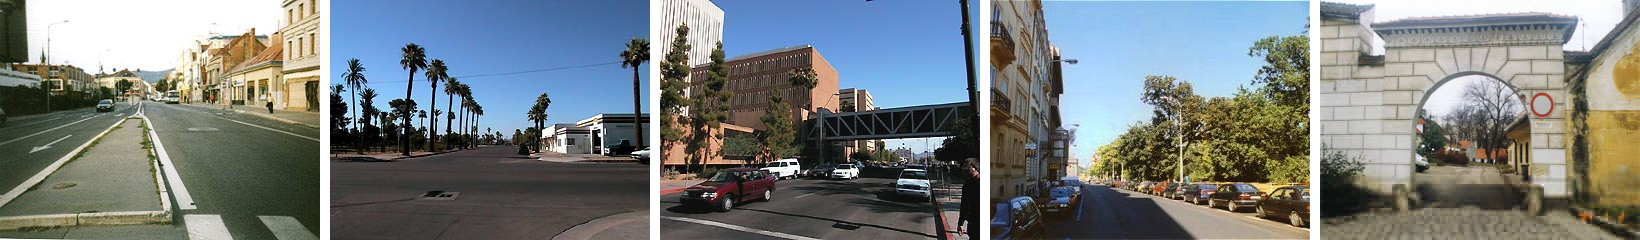
\includegraphics[width=\textwidth]{img/inriaNegatives.png}
		\caption{Negatives}
		\label{fig:inriaNegatives}
	\end{subfigure}
	\caption{Example INRIA images.}
	\label{fig:inriaExampleImages}
\end{figure}

\subsection{Deficiencies \& pitfalls}
10 duplicate negative train images

Occluded or small persons in negatives

Duplicates:
1 neg test
10 neg train

\section{Example}

\begin{figure}
	\centering
	\begin{subfigure}[t]{\textwidth}
		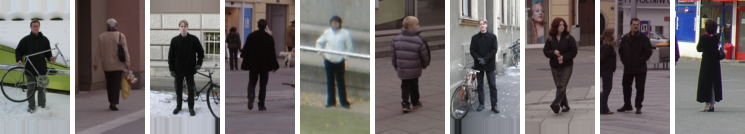
\includegraphics[width=\textwidth]{img/objectDetectionTP.png}
		\caption{True positives}
		\label{fig:objectDetectionTP}
		\vspace{2mm}
	\end{subfigure}
	\begin{subfigure}[t]{\textwidth}
		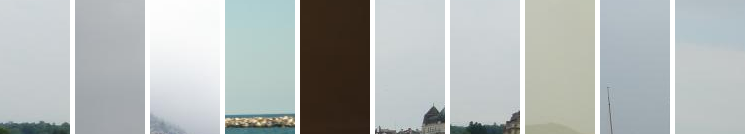
\includegraphics[width=\textwidth]{img/objectDetectionTN.png}
		\caption{True negatives}
		\label{fig:objectDetectionTN}
		\vspace{2mm}
	\end{subfigure}
	\begin{subfigure}[t]{\textwidth}
		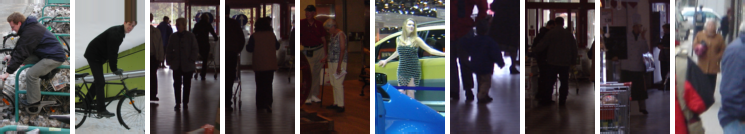
\includegraphics[width=\textwidth]{img/objectDetectionFN.png}
		\caption{False negatives}
		\label{fig:objectDetectionFN}
		\vspace{2mm}
	\end{subfigure}
	\begin{subfigure}[t]{\textwidth}
		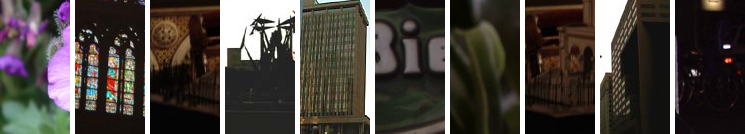
\includegraphics[width=\textwidth]{img/objectDetectionFP.png}
		\caption{False positives}
		\label{fig:objectDetectionFP}
	\end{subfigure}
	\caption{Example classifications of INRIA windows.}
	\label{fig:imageCorrespondenceCurves}
\end{figure}

\section{Parameter study}
\label{sec:odParameterStudy}

\subbibliography

\end{document}
